\documentclass[../../main]{subfiles}
\begin{document}
\subsection{Overall system architecture}
The system is divided in two main part:
    \begin{itemize}
        \item An Android Client;
        \item A Server, divided in:
        \begin{itemize}
            \item Nodejs Server;
            \item Python Server (only internal use);
        \end{itemize}
    \end{itemize}
A overall picture describing the architecture is avaible at\ \ref{system_architecture}.

\paragraph*{Authentication}
The client authenticate via google account with Firebase Auth API, generating his token and sending it to the server 
that will generate a token with the user email and control if they match. After this the client sends 
his \textbf{Notification token} and his \textbf{Public key} to the server that will store them in the user collection on firebase.

\paragraph*{RESTful APIs}
The clients and the Nodejs server communicate via RESTful APIs, but the server can also send FCM message, received as push notification, to the client.
The APIs used allow the user to manage his data:

\begin{itemize}
    \item Points of Interest \textbf{'/points-of-interest'}:
    \begin{itemize}
        \item \textbf{'/'} Get pois list (GET);
        \item \textbf{'/add'} Add a poi (POST);
        \item \textbf{'/remove'} Remove a poi (DELETE);
    \end{itemize}

    \item Live Events \textbf{'/live-events'}:
    \begin{itemize}
        \item \textbf{'/'} Get live events list (GET);
        \item \textbf{'/add'} Add a live event (POST);
    \end{itemize}

    \item Friends \textbf{'/friends'}:
    \begin{itemize}
        \item \textbf{'/'} Get friends list (GET);
        \item \textbf{'/add'} Add a friend request (POST);
        \item \textbf{'/confirm'} Confirm a friend request (POST);
        \item \textbf{'/deny'} Deny a friend request (POST);
        \item \textbf{'/remove'} Remove a friend (DELETE);
    \end{itemize}

    \item Recommendation \textbf{'/recommendation'}:
    \begin{itemize}
        \item \textbf{'/places'} Places (POST);
        \item \textbf{'/validity'} Validity (POST);
        \item \textbf{'/train'} Train (POST)
    \end{itemize}

    \item Authentication \textbf{'/user-data'}:
    \begin{itemize}
        \item \textbf{'/notification-token'} Save notification token (POST);
        \item \textbf{'/public-key'} Save user RSA public key (POST);
        \item Train (POST)
    \end{itemize}

\end{itemize}
    \begin{figure}[h]
        \centering
        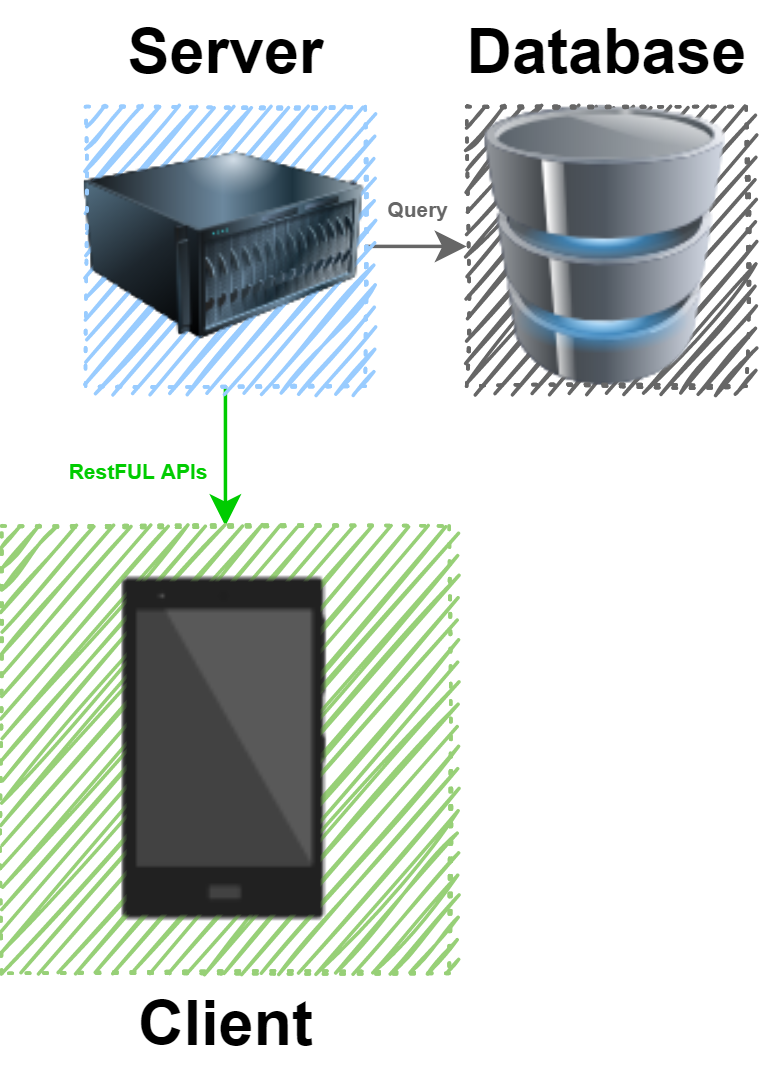
\includegraphics[width=100mm,height=130mm]{images/simple.png}
        \caption{System Architecture}\label{system_architecture}
    \end{figure}

\paragraph*{Server}

The server is made of two component, a Nodejs server and a Python server.
The Node server is used to handle the communication with:
\begin{itemize}
    \item Firestore Database, via Firebase APIs;
    \item Android Client, via RESTful APIs and FCM;
    \item Python Server, via Internal RESTful APIs;
\end{itemize}
The server retrieves and manipulate, on request of the user, data from the \textbf{Firestore Database}, 
asks a recommendation to the model based on the \textbf{Python Server} 
and sends the data that the client asked via RESTful APIs or sends \textbf{FCM} message as \textbf{Push Notification} to the \textbf{Android Client}.


\end{document}